% 12pt .6pt grayscale fragment; standalone tikz; no document env
\usetikzlibrary{arrows.meta,calc}
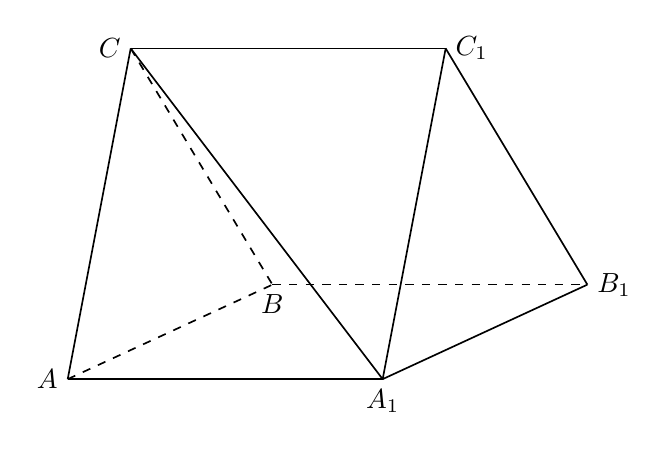
\begin{tikzpicture}[line width=0.6pt,>=Stealth,font=\normalsize]
\coordinate (A) at (0,0);
\coordinate (Aone) at (4,0);
\coordinate (B) at (2.6,1.2);
\coordinate (C) at (0.8,4.2);
\coordinate (Cone) at (4.8,4.2);
\coordinate (Bone) at (6.6,1.2);
\draw (A)--(Aone);
\draw (Aone)--(Bone);
\draw (Bone)--(Cone);
\draw (Cone)--(C);
\draw (C)--(A);
\draw (C)--(Cone);
\draw (Aone)--(Cone);
\draw (Aone)--(C);
\draw[dashed] (A)--(B);
\draw[dashed] (C)--(B);
\draw[dashed] (B)--(Bone);
\node[left] at (A) {$A$};
\node[below] at (B) {$B$};
\node[left] at (C) {$C$};
\node[below] at (Aone) {$A_{1}$};
\node[right] at (Bone) {$B_{1}$};
\node[right] at (Cone) {$C_{1}$};
\end{tikzpicture}
